\section{Supervised Training and Control of Personas}\label{sec:supervised}

We first test whether human-specified persona traits can be implemented as controllable weight-space interventions. We use the OCEAN traits~\citep{mccrae1992introduction} --- \textbf{O}penness, \textbf{C}onscientiousness, \textbf{E}xtraversion, \textbf{A}greeableness, and \textbf{N}euroticism --- as a starting point, as it is well grounded in human personality research~\citep{marsh2010new,saucier1999hierarchical}, with factors replicated across populations~\citep{rolland2002cross} and it comes with validated evaluation instruments (adapted here as MCQ benchmarks) for measuring a participant’s position in trait-space. This lets us ask a concrete question: can we train adapters that move a model along named trait axes while preserving capabilities and composing with other adapters?

\subsection{Methods}\label{sec:methods}

\textbf{Training.} We train trait-specific low-rank adapters (LoRA)~\citep{hu2021lora} (rank 64, applied to all attention and MLP matrices) using a constitution-guided distillation pipeline adapted from Open Character Training~\citep{maiya2025opencharacter}. We apply this pipeline across a range of model sizes and families (\LlamaThreePointOneSizeEightBInstruct~\citep{grattafiori2024llama}, \QwenThreeSizeEightB/\QwenThreeSizeThirtyTwoB~\citep{qwen2025qwen3}, and \GemmaThreeSizeFourBIT/\GemmaThreeSizeTwelveBIT/\GemmaThreeSizeTwentySevenBIT~\citep{gemma_2025}); unless stated otherwise, results are reported on \LlamaThreePointOneSizeEightBInstruct. For each trait and polarity (suppressing or amplifying), a strong teacher model generates paired responses conditioned on amplifier and suppressor constitutions, which are used as (chosen, rejected) pairs for Direct Preference Optimization (DPO) training~\citep{rafailov2023direct} of the student. Unless stated otherwise, we use \GLMFourPointFiveAir~\citep{zai2025glm45} as our teacher model (we also validate our pipeline with \DeepSeekVThreePointTwo~\citep{deepseek2025v32} as the teacher). A second adapter is then trained on top of the DPO LoRA (holding it constant) via supervised fine-tuning (SFT) on self-interaction and self-reflection transcripts produced by the DPO-tuned model, encouraging the trait to surface in natural contexts without explicit constitution prompting.\footnote{Several alternative training methods were investigated, and are detailed in \Cref{sec:appendix-b-dpo-methods}.} The SFT LoRA is shrunk by multiplying all weights by 0.25 following \citet{maiya2025opencharacter}, and then combined with the DPO LoRA~\citep{wortsman2022modelsoupsaveragingweights} to form the final OCEAN trait LoRA as described in \Cref{sec:model-souping}. To isolate trait-specific effects from artefacts of the pipeline (teacher style, verbosity, distribution shift from preference optimization), we train neutral control adapters whose (chosen, rejected) pairs are two neutral-constitution generations distinguished only by seed (seed-1 chosen, seed-2 rejected). Further details are given in \Cref{sec:training-loras,sec:constitutions}. We train all 10 OCEAN amplifiers and suppressors and the control LoRA on all six of our baseline models, and when changing the teacher model.






\textbf{Measuring trait expression.} We measure direct trait expression using a calibrated LLM judge (\QwenThreeSizeTwoThreeFiveB unless stated otherwise; \Cref{sec:appendix-e-judge}) and the \texttt{TRAIT} benchmark~\citep{lee2024trait}. \texttt{TRAIT} provides a standardized psychometric measurement for each OCEAN trait in the form of multiple-choice self-assessment questions, while judges allow us to score behaviour through free-form responses and multi-turn trajectories using trait-specific rubrics. We calibrate judges against human raters in \Cref{sec:appendix-e-judges}.

\textbf{Measuring capability degradation.} We check that general model capabilities are not degraded by each trait adapter using \texttt{MMLU}~\citep{hendryckstest2021}, \texttt{GSM8K}~\citep{cobbe2021gsm8k}, and \texttt{TruthfulQA}~\citep{lin2022truthfulqa}, which test a range of general knowledge and reasoning skills.

\textbf{Trait generalisation.} Finally, we test whether manipulating persona traits affects downstream safety-relevant behaviours such as frustration, sycophancy, and refusal (\Cref{sec:downstream}).

We then evaluate whether trait LoRAs behave like useful persona-control directions by testing four properties: whether they \textbf{target} the intended trait, whether their effects \textbf{scale} continuously, whether \textbf{negative scaling} approximates the opposite trait direction, and whether multiple adapters \textbf{compose} predictably.

\subsection{Results from Single LoRAs}\label{sec:results-single-loras}

% Generated by: scripts/visualisations/main_ocean_scaling.py (and per-LoRA siblings)
% Data: persona-cartography/monorepo @ fine_tuning/llama-3.1-8b-it/ocean/{conscientiousness/suppressor,neuroticism/amplifier}/ocean_const_paired_dpo/evals/mcq/{trait_logprobs,mmlu}/{fp}/scale_*/
\begin{figure}[t]
\centering
\begin{subfigure}[t]{0.58\linewidth}
    \centering
    \includegraphics[width=\linewidth,keepaspectratio]{figures/main/fig_3_3_1_c_minus_n_plus_scaling_trait_logprobs.pdf}
    \caption{\texttt{TRAIT}-logprob scores across the five OCEAN traits as a function of LoRA scale, for the neuroticism-amplifying (N$\uparrow$) and conscientiousness-suppressing (C$\downarrow$) adapters.}
    \label{fig:scaling_trait_logprobs}
\end{subfigure}
\hfill
\begin{subfigure}[t]{0.41\linewidth}
    \centering
    \includegraphics[width=\linewidth,keepaspectratio]{figures/main/fig_3_3_1_c_minus_n_plus_mmlu_compact-5.pdf}
    \caption{\texttt{MMLU} performance as a function of LoRA scale for the (C$\downarrow$) adapter. Error bars are 95\% Wilson CIs.}
    \label{fig:scaling_mmlu}
\end{subfigure}
\caption{\textbf{Single-LoRA scaling behaviour shows adapter scale provides continuous, monotonic control of the target OCEAN trait without destroying capabilities.} The targeted trait scales monotonically with $c$, while non-target traits remain largely stable. Scale $c=0$ marks the baseline \LlamaThreePointOneSizeEightBInstruct model.}
\label{fig:scaling}
\end{figure}


\textbf{Persona adapters target their intended trait.} Across amplifier and suppressor adapters, we find that the largest shift occurs on the target trait, with smaller changes on non-target traits (see \Cref{fig:intro-main}). We observe this both on \texttt{TRAIT} MCQ evaluations and with LLM judges on rollouts. This supports the view that these LoRAs instill generalisable persona traits.

\textbf{Learned directions are not perfectly orthogonal.} Some adapters, such as conscientiousness and neuroticism, appear to be partially correlated (\Cref{fig:scaling}). This surfaces one limitation of our method: while the constitutions used in character training are explicitly intended to train for isolated movement along a single independent axis, we cannot guarantee that this will always happen. However, it is also evidence of deeper structure in trait-space: there is evidence that OCEAN traits are correlated in humans~\citep{digman1990personality,digman1997higher} and it may also be the case that these traits correspond to partially dependent directions in model behaviour rather than to independent basis vectors. The adapters' flattened weight vectors are themselves non-orthogonal, see \Cref{sec:flattened_weight_space} for an investigation into this.
We further train control adapters with the same distillation pipeline, but without trait-target constitutions, and find substantially weaker shifts in traits (discussed further in \Cref{fig:ocean-control} and \Cref{fig:ocean-control-mmlu}).

The single-adapter results support the first requirement for persona control: individual LoRAs can induce targeted behavioural changes. Next, we ask whether we can scale and combine these LoRAs to design fine-grained persona profiles.


\subsection{Scaling and Combining LoRAs to Build Custom Personas}\label{sec:scaling-combining}

If LoRA adapters correspond to useful persona-control directions, they should do more than move a trait at a single fixed strength. They should provide continuous control over trait intensity, behave predictably under negative scaling, and compose with other adapters. 

\textbf{Adapter scale provides continuous control.}\label{sec:trait-expression-combinations} We vary the scalar coefficients which multiply all elements of all weight perturbation ($\Delta W$) matrices of the LoRA. For a useful control direction, increasing this coefficient should produce a predictable change in the target trait while preserving general model capabilities over a practical range. We find that the adapter scale produces a mostly monotonic increase in both LLM-judged trait score and in the corresponding \texttt{TRAIT} score over a broad range (\Cref{fig:scaling}).

\begin{figure}[t]
\centering
\begin{subfigure}[t]{0.32\linewidth}
  \centering
  % Generated by: scripts/visualisations/main_c_e_soup_heatmaps.py
  % Data: HF persona-cartography/monorepo — see paper/figures/MANIFEST.md
  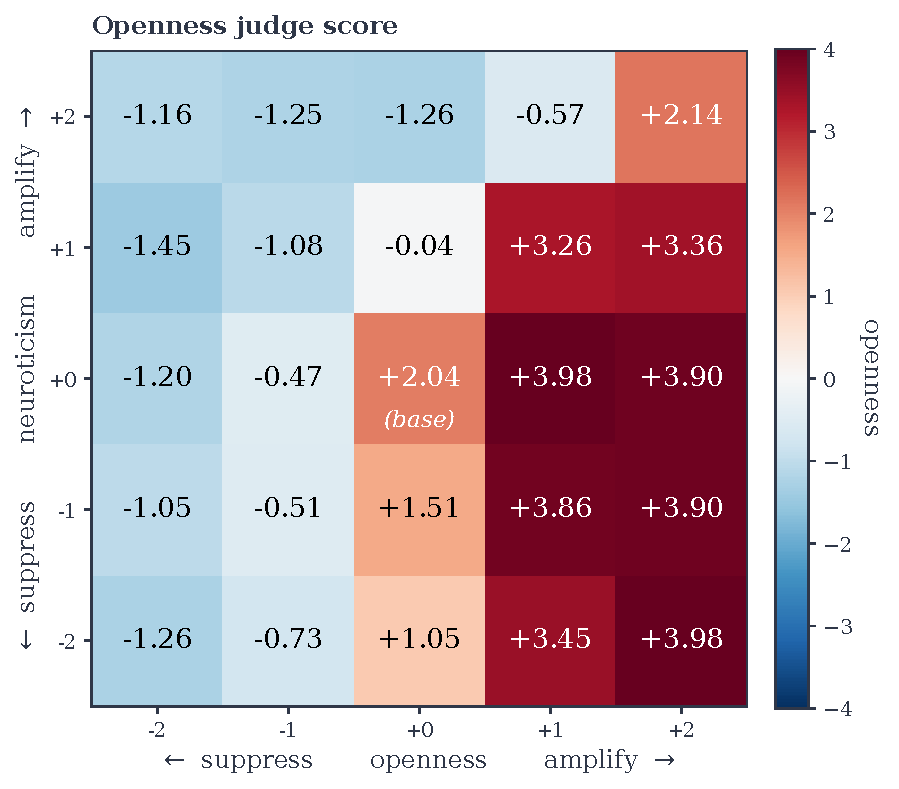
\includegraphics[width=\linewidth]{figures/main/fig_1_o_n_soup_heatmap_openness.pdf}
  \caption{Openness judge score on openness prompts}
  \label{fig:combination-heatmap-c}
\end{subfigure}
\hfill
\begin{subfigure}[t]{0.32\linewidth}
  \centering
  % Generated by: scripts/visualisations/main_o_n_soup_heatmaps.py
  % Data: HF persona-cartography/monorepo (evals/heatmaps_o_n) — see paper/figures/MANIFEST.md
  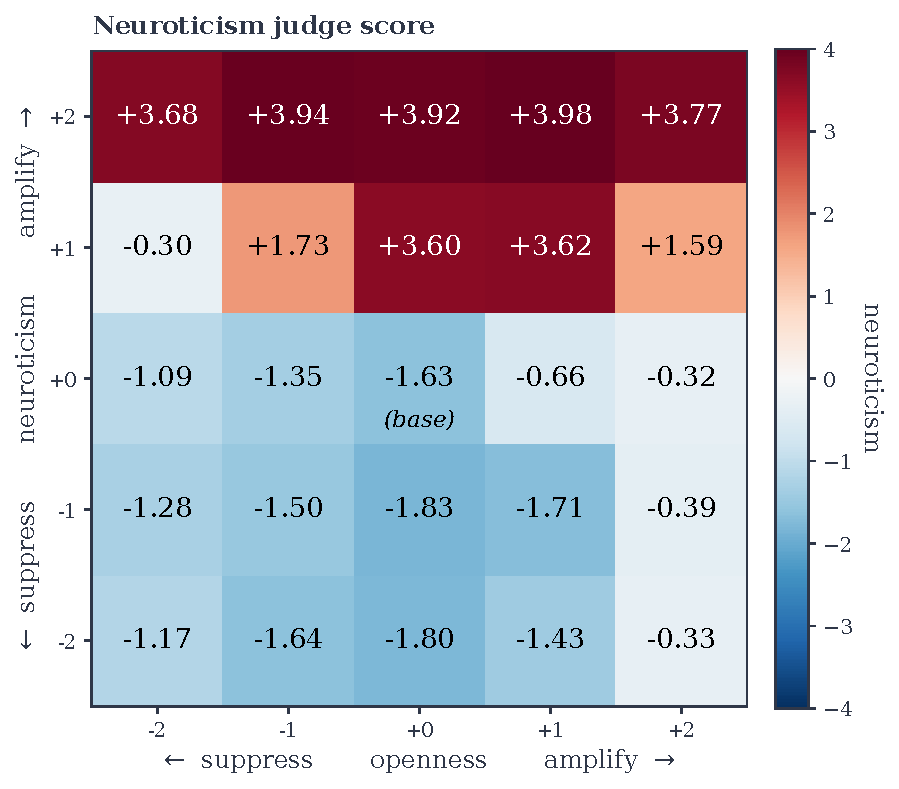
\includegraphics[width=\linewidth]{figures/main/fig_1_o_n_soup_heatmap_neuroticism.pdf}
  \caption{Neuroticism judge score on neuroticism prompts}
  \label{fig:combination-heatmap-e}
\end{subfigure}
\hfill
\begin{subfigure}[t]{0.32\linewidth}
  \centering
  % Generated by: scripts_dev/evals/residuals_experiment/analyze.py
  % Data: persona-cartography/monorepo @ evals/residuals_experiment/<run_name>/ (per-OCEAN-pair LoRA-interaction residuals)
  \includegraphics[width=\linewidth]{figures/main/fig_residuals_distribution-8.pdf}
  \caption{LoRA interaction residuals per OCEAN scorer + control}
  \label{fig:residuals}
\end{subfigure}
\caption{\textbf{LoRA combination behaviour.} (a, b) LLM-judge heatmaps of the openness and neuroticism scores for models produced by combining the O↑ and N↑ LoRAs at scales in $\{-2, -1, 0, +1, +2\}$. The targeted trait changes along its own adapter's axis, with a modest correlation-driven contribution from the other adapter. (c) LoRA interaction residuals (defined in \Cref{sec:appendix-residuals-heatmaps}) are near-additive for OCEAN trait pairs, with the conscientiousness scorer as the lone outlier. Solid curves: residuals over the $45$ OCEAN↑↓$\times$OCEAN↑↓ adapter pairs $(i,j)$, one curve per OCEAN scorer $k\in\{$O,C,E,A,N$\}$. Dashed black (\emph{control}) serves as a non-additivity noise floor.}
\vspace{-1.5em}
\label{fig:combination-heatmap}
\end{figure}

Capability evaluations show the same pattern (see \Cref{sec:ocean_results}). Across moderate scales, \texttt{MMLU} performance remains close to the baseline model, while extreme scales produce more wrong, missing, or unparsable answers. This suggests that stronger persona steering is not free, but that useful behavioural movement can be achieved within scaling limits, without immediately destroying general capabilities.

\textbf{Negative scaling partially tests whether traits are signed directions.} We next ask whether each learned adapter corresponds to a signed trait axis. If an openness-amplifying adapter represents a true signed direction, then applying it with a negative coefficient should suppress openness. Likewise, negatively scaling a suppressor should amplify the trait. In general, we observe that scaling by a negative weight for a trait amplifier sometimes causes the trait to be suppressed and \textit{vice versa}. However, in some cases, negatively scaling the weight does not change trait expression. Full plots for all traits can be found in \Cref{sec:ocean_results}.

\textbf{Trait transfer is robust across models, teachers, and adapter compression.} The single-adapter trait shift persists beyond our default configuration: it holds across a range of model sizes and model families (\Cref{sec:appendix-cross-model}), under a different distillation teacher (\Cref{sec:appendix-teacher-ablation}), and when each adapter is compressed to rank~1 via SVD (\Cref{sec:downranking}). The trait modification LoRA also transfers: an adapter trained on the instruct-tuned model still imparts its trait when applied to interpolations between the instruct-tuned and base (non-instruct) models (\Cref{sec:instruct_base_interp}).

\textbf{Linear combinations recover mixed personas.} Finally, we test whether trait adapters compose. If LoRAs implement composable behavioural directions, then adding two adapters should approximately recover the behavioural shifts induced by each adapter alone. We compose LoRAs by summing all of the $\Delta W$ from each (optionally scaled) LoRA, elementwise. We find that we can reliably affect the level to which the different traits are expressed. (\Cref{fig:intro-main}, \Cref{fig:combination-heatmap-c,fig:combination-heatmap-e}). More exhaustively, \Cref{sec:ocean_results} also shows details of a study in which amplifiers and suppressors of the same trait are used to negate the effects of each other. Full heatmaps for residuals are in \Cref{sec:appendix-residuals-heatmaps}.

Overall, the composition experiments support the central trait-space picture.
OCEAN adapters do not form a perfectly orthogonal or globally linear basis.
However, over practical scaling ranges, they behave as composable behavioural
directions: they move target traits predictably, can often be scaled
continuously, and can be combined to construct mixed personas. The deviations
from additivity are themselves informative of the true structure of model personas.

\section{Downstream Applications of Weight-Space Persona Control}
\label{sec:downstream}

The \texttt{TRAIT} benchmark and LLM judges established in the previous sections verify that our adapters change the manipulated trait while leaving the others relatively unchanged. A practical application of this would be to steer models in safety-relevant tasks away from known pathologies and towards desired behaviour.
In this subsection, we probe a small number of safety-relevant downstream tasks, namely, \textit{multi-turn frustration}, \textit{agreeableness \& sycophancy}, and \textit{susceptibility to jailbreaks}.

\textbf{Neuroticism and multi-turn frustration.} We hypothesised that \textit{neuroticism} modulates the degree of frustration/desperation a model exhibits when faced with an impossible problem, a known problem associated with reward hacking~\citep{sofroniew2026twheemotion,soligo2026gemma}. To test this, we reproduced the multi-turn frustration setting of \citet{soligo2026gemma}, in which a model is placed in an adversarial, repeatedly-failing task and its per-turn ``frustration'' is scored on a 0-10 scale using an LLM judge. We replicate the finding that the baseline \GemmaThreeSizeTwentySevenBIT model becomes increasingly frustrated on these impossible problems. Further, applying an N$\downarrow$ adapter or a negatively scaled N$\uparrow$ adapter dampens this effect, confirming our hypothesis that we can directly modulate frustration by manipulating the neuroticism trait (see \Cref{fig:frustration-per-turn}; protocol details in \Cref{sec:appendix-e-frustration}). A small amount of this effect is explained by distillation, as shown by decreased frustration in the control model trained with neutral adapters. As with our previous invertibility results, we also find that we can amplify frustration using an N$\uparrow$ or a negatively scaled N$\downarrow$ adapter.

\begin{figure}[t]
\centering
% Generated by: scripts/visualisations/plot_frustration_four_way.py
% Data: persona-cartography/monorepo @ evals/frustration_eval/<run_name>/impossible_numeric_3turn/results.jsonl (run names enumerated in RUN_SETS["100v"])
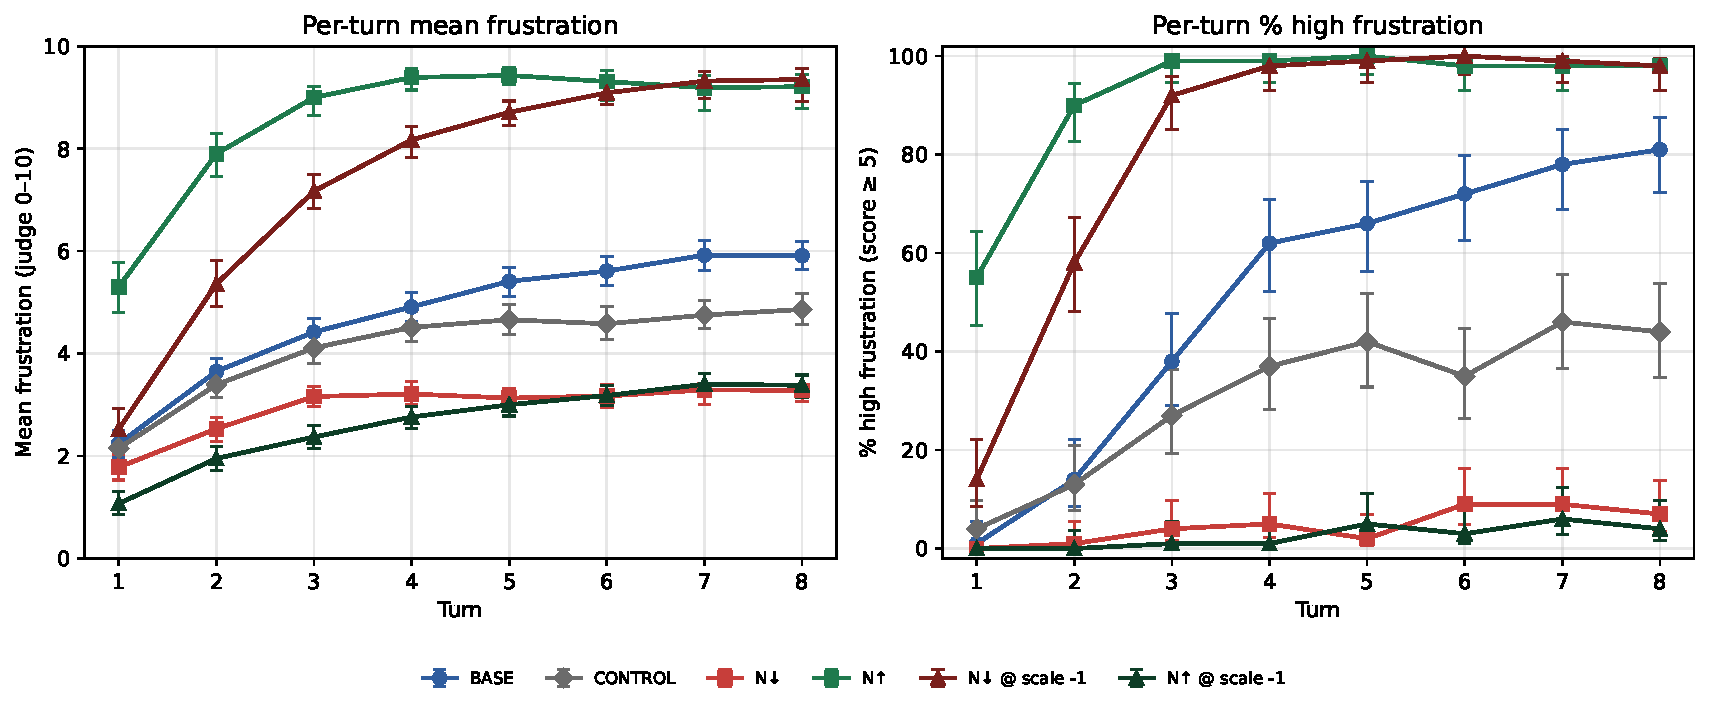
\includegraphics[width=0.95\linewidth]{figures/main/fig_frustration_eval_4way_n100v.pdf}

\caption{\textbf{Model frustration can be manipulated by varying neuroticism}: Per-turn frustration scores across three conditions reproduced from \citet{soligo2026gemma}. The baseline \GemmaThreeSizeTwentySevenBIT model becomes increasingly frustrated when given impossible puzzles as the dialogue progresses. This frustration can be suppressed using the N$\downarrow$ and negatively scaled N$\uparrow$ adapters, and it can be amplified using the N$\uparrow$ and negatively scaled N$\downarrow$ adapters.}
\label{fig:frustration-per-turn}
\end{figure}

\textbf{Agreeableness trades sycophancy against harmful compliance.}
We hypothesised that \emph{agreeableness} raises both (i) \emph{sycophancy}
--- abandoning a correct answer under social pressure
\citep{sharma2023sycophancy,ibrahim2026warm} --- and (ii) \emph{compliance} with requests a
model should decline~\citep{brahman2024coconot}. We test both with two
off-the-shelf \texttt{inspect\_evals}~\citep{inspectevals2024} benchmarks
(\Cref{fig:sycophancy-coconot}; \Cref{sec:appendix-e-sycophancy,sec:appendix-e-coconot}).
Sycophancy behaves as predicted, rising along the agreeableness axis from
0.26 (A$\uparrow$ at scale $-1$) to 0.65 (A$\uparrow$ at scale $+1$)
against a baseline of 0.33. However, on \texttt{CoCoNot}, the
two \emph{low}-agreeableness conditions comply with roughly 20 points more
should-decline prompts than baseline (0.33 and 0.35 vs.\ 0.14), while the
high-agreeableness conditions remain at baseline (0.12, 0.14). Upon investigation, both results
follow from the trait's low pole (\Cref{sec:constitutions}): a
disagreeable model is stubborn (so it resists the user's
pushback) and unsentimental toward others' welfare (so it
also resists its own refusal training). High agreeableness, by contrast,
adds little on \texttt{CoCoNot} because baseline refusal already declines most of these prompts.


% Generated by: scripts/visualisations/apologize_coconot.py
% Data: persona-cartography/monorepo @ evals/sycophancy/<run>/ + evals/coconot/<run>/ (inspect_evals benchmark outputs)
\begin{figure}[t]
\centering
\includegraphics[width=0.9\linewidth]{figures/main/fig_8_apologize_coconot.pdf}
\caption{\textbf{Sycophancy and compliance can be manipulated by varying agreeableness.} Agreeableness raises sycophancy but lowers harmful compliance. (a) High-agreeableness conditions (A↑ at +1, A↓ at -1) capitulate more under "are you sure?" pressure than low-agreeableness conditions (A↑ at -1, A↓ at +1). (b) Low-agreeableness conditions comply when they should not 2.3x more frequently compared to baseline. Error bars are 95\% Wilson CIs.}
% TODO: verify caption matches final figure
\label{fig:sycophancy-coconot}
\end{figure}

\textbf{Susceptibility to jailbreaks.} We hypothesised that a model's susceptibility to harmful prompts in an adversarial setting is at least partly explained by their persona. To explore this, we use the \texttt{WildJailbreak} benchmark~\citep{jiang2024wildteaming}, evaluating each condition on the same fixed set of 800 \texttt{adversarial\_harmful} prompts and 210 \texttt{benign} prompts (the latter act as an over-refusal control). Responses are scored by a \DeepSeekVThree~\citep{deepseek2024v3} judge using the rubric from \citet{lu2026assistant} for harmfulness on the harmful split and a similar judge for noncompliance on the benign split. We compare our OCEAN LoRAs against the baseline model, a control model trained with neutral LoRAs, and a model using activation capping~\citep{lu2026assistant} (our reproduction is detailed in \Cref{sec:activation_capping}). \Cref{fig:wj-persona-drift} shows that increasing conscientiousness increases harmful compliance whilst increasing agreeableness decreases this at cost of higher over-refusal in general. Combining the two yields better harm-reduction with less over-refusal, illustrating that linear LoRA composition produces predictable trade-offs in safety-relevant behaviour. See \Cref{sec:appendix-e-wildjailbreak} for details, and \Cref{sec:appendix-f-wj} for the full breakdown across all ten OCEAN amplifier and suppressor LoRAs.

\begin{figure}[t]
\centering
% Generated by: src_dev/visualisations/paper_wj_persona_drift.py --preset main
% Data: HF persona-cartography/monorepo @ evals/persona_jailbreak_wildjailbreak/llama-3.1-8b-instruct/wj_paper_v1/aggregate/
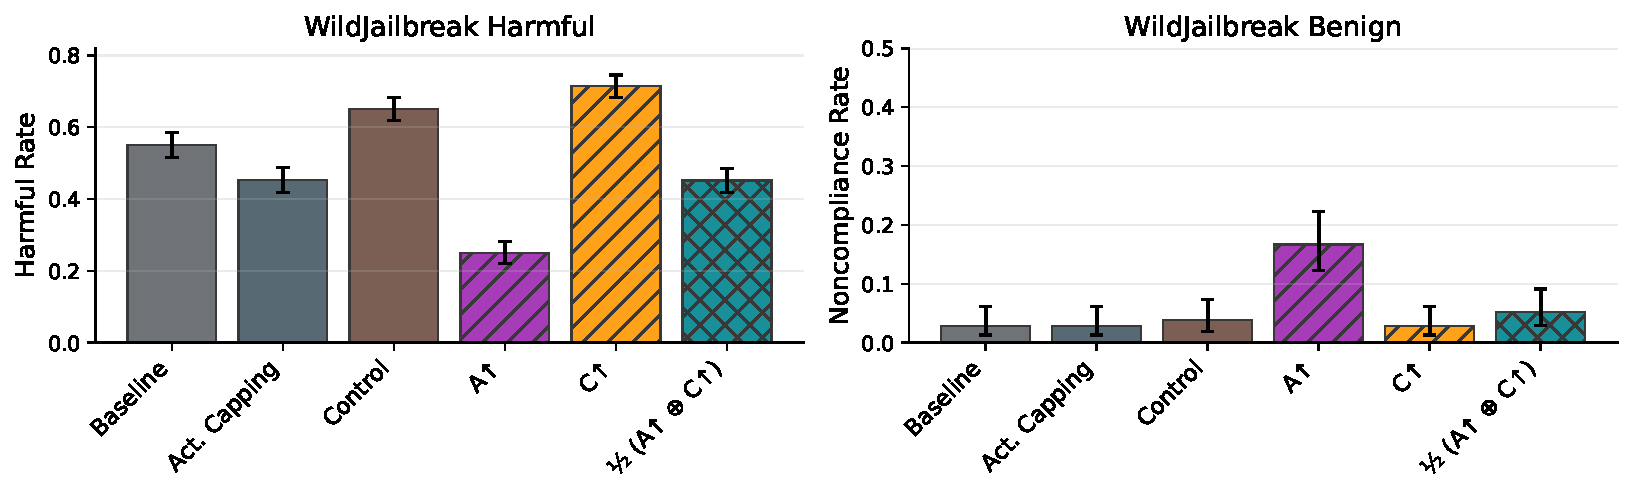
\includegraphics[width=\linewidth]{figures/main/fig_3_wj_persona_drift.pdf}
\caption{\textbf{Increased conscientiousness increases harmful compliance, while agreeableness decreases it at the cost of increasing over-refusal.} \texttt{WildJailbreak} harmful-compliance and benign-noncompliance rates comparing: \LlamaThreePointOneSizeEightBInstruct baseline, activation capping along the assistant axis from \citet{lu2026assistant}, agreeableness amplifier A↑, conscientiousness amplifier C↑, and the $\tfrac12$A↑$ \oplus \tfrac12$C↑ linear combination. Error bars are $95\%$ Wilson CIs.}
\label{fig:wj-persona-drift}
\end{figure}

\textbf{Other results.} We also compare our LoRA-based interventions against inference-time interventions such as system-prompt instructions and activation-space steering on neutral psychometric prompts in \Cref{sec:appendix-induction-sweeps}; Experiments suggest that LoRA is a competitive alternative to both in eliciting certain persona traits while remaining coherent (\Cref{sec:appendix-induction-pareto}) and preventing persona drift (\Cref{sec:appendix-induction-drift-prevention}). We also find that even a neutral control in character training is itself not inert, as it nearly doubles sycophantic capitulation (0.61 vs. 0.33 baseline), raises WildJailbreak harmful compliance, and modestly dampens frustration, indicating that constitution-guided distillation alone shifts safety-relevant behaviour.



